% !TEX root =  GroupDet.tex
\section{Experiments}
\label{expall}

We evaluate our approach on three distinct datasets, two that involve humans and one that involves mice. This tests the generality of our framework because the datasets are very different from one another, with distinct types of individual and pairwise descriptors in each case.that are appropriate for each case are quite different. Due to space constraints, the following discussion is brief. Additional details and experimental results can be found in the accompanying supplemental material.

\vspace{0.05in}\noindent\textbf{Classroom Interaction Database.} We collected and annotated a new database of videos capturing students' behaviors over five hour-long sessions in an interactive classroom at a major university. As shown in the left-most images of Fig.~\ref{retrieved}, the students are seated in a regular lecture hall and are observed by a camera array with non-overlapping fields of view. The classroom is ``interactive'' because at various times throughout the lecture students are invited to engage in ad-hoc group discussions about problems provided by the instructor (see, e.g.,~\cite{Crouch:PI}). The ad-hoc groups can form within and across seating rows, and detecting them is a challenge because the number of by-standers  is much larger than the number of participants ($M$ is between 10 and 20 while $N$ is between 2 and 4), video quality is limited (low light, less than 15fps), and the visual cues for interaction are quite subtle. The ability to automatically detect such interactions is important for education researchers, however, since it can help in understanding how students self-organize into groups, and which geometric configurations of groups lead to improved educational outcomes.

Through a combination of face detection and tracking, we obtained noisy tracks for all students in each monocular video. We manually identified the participants and start/end times of all two-person, three-person, and four-person interactions, obtaining 254 two-person, 112 three-person, and 16 four-person interactions in total. In consultation with education experts we define interaction categories based on the geometric configurations of the participants: three categories for 2-person interactions (same row; different rows with left agent in front; different rows with right agent in front) and four categories for 3-person interactions. Details and example images for each category can be found in the accompanying supplemental material. The annotated interactions range from a few seconds to tens of seconds in length. Since the raw videos arise from five different hour-long session, and we adopt a leave-one-session-out evaluation scheme in partitioning  training samples (exemplars) from test samples (inputs). Also, for each split of the data we manually eliminate the false detections and tracks in the exemplars, while leaving them present in the test samples. 

\begin{figure*}
\begin{center}
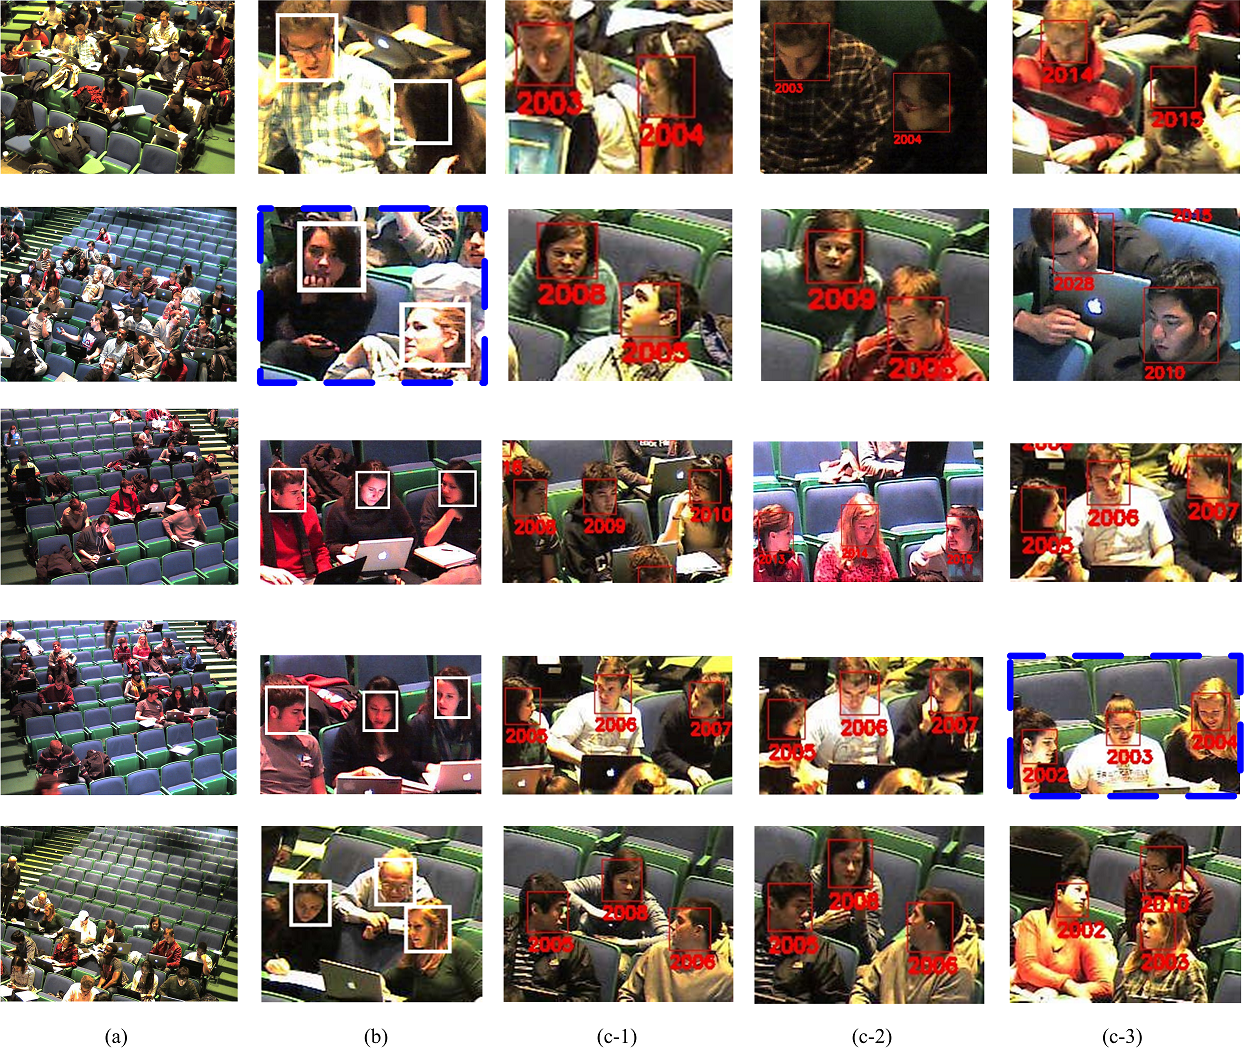
\includegraphics[scale=2.25]{retrieved.png}
\end{center}
\vspace{-10pt}
\caption{Examples of social interaction detection and matching on the classroom interaction database. Each row is an example of detecting a salient interaction from an input and enumerating similar database exemplars: (a) is the input, (b) is the detected social interaction, and (c-1) to (c-3) are the top three associated database exemplars that support this detection.\todd{Can you remove the right-most column of images (and thus the fourth row) and make this into a single-column figure? You could still include the full five-column version in the supplemental material.}}
\label{retrieved}
\end{figure*}

We use four-level temporal pyramids for the interactions and set the time unit to be half the duration of the cells in the lowest level. For individual descriptors we use nine-dimensional vectors that crudely encode the agents' head pose, and for pairwise descriptors we use vectors of dimension $2(N-1)$ that encode, in a manner invariant to similarity transforms, the location of an agent relative to all other $(N-1)$ participants. More details can be found in the supplemental material.

We begin by looking at accuracy of detection, where we ignore the inferred interaction categories and simply measure the systems ability to detect when an interaction has occurred. Figure~\ref{ROC} shows detection ROC curves for different group sizes with various parts of the system turned off. This includes using only one of the individual or pairwise descriptors, and using metric learning (optimized $\Sigma_I,\Sigma_P$) or not ($\Sigma_I$ and $\Sigma_P$ set to identity matrices). Using all parts of the system yields the best results, and we note that performance improves as the number of participants $N$ increases. The latter is due to the fact that interaction patterns are more easily discriminated when more pairwise information is available.
%t is interesting that pairwise descriptor performs better than individual descriptor, mainly due to the fact that the interaction only occur among nearby students in a classroom environment and therefore geometric context provides a strong clue for a potential occurrence of interaction. 

\begin{figure*}[t]
\begin{center}
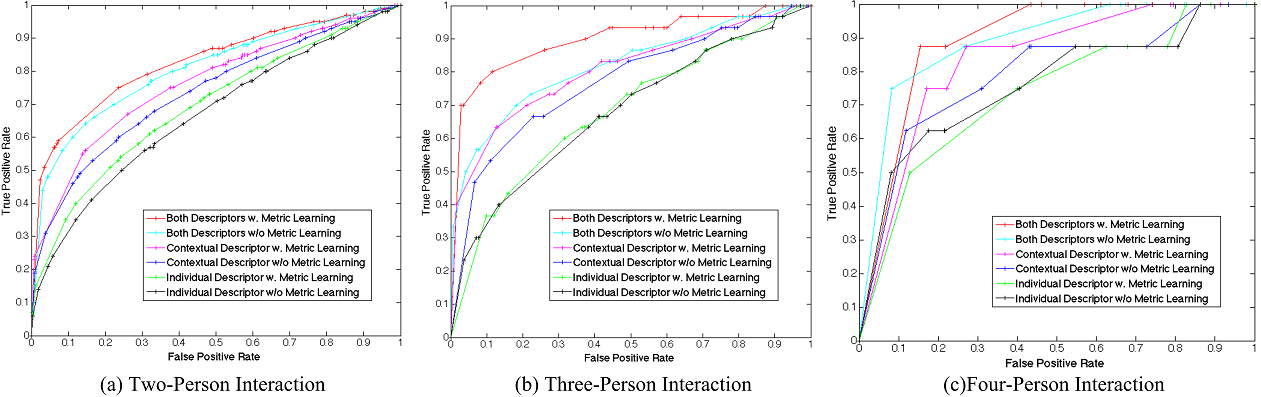
\includegraphics[scale=2.5]{ROC.png}
\end{center}
\caption{ROC curves for identifying the participants of an two-person, three-person, and four-person interactions using the proposed approach and baselines. \todd{You could move the $N=3$ graph to the supplemental material and make this a single-column figure.} }
\label{ROC}
\end{figure*}


\begin{figure*}[t]
\begin{center}
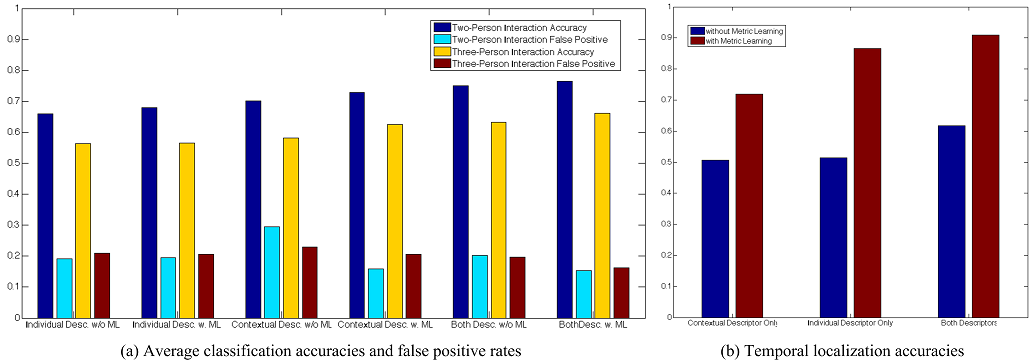
\includegraphics[scale=2.5]{classtemporal.png}
\end{center}
\caption{Average classification accuracies and false positives for two-person and three-person interactions (Individual and/or pairwise descriptors, with or without metric learning (ML)) and the temporal localization accuracies.\todd{Remove temporal localization and make this a single-column figure.}}
\label{classtemporal}
\end{figure*}

Next, we study classification performance for 2-person and 3-person interactions, where we measure the accuracy of inferred interaction categories (due to the small number of 4-person interactions in our dataset, we did not define categories for them). As before we do this with various parts of the system turned off, and Fig.~\ref{classtemporal} shows for all correctly-detected interactions the average true positive rates vs. false positives when further classifying them into the three or four categories. \todd{I do not understand the previous sentence.} Again we see that performance improves when more parts of the system turned on. We can also draw a contrast with the detection results of Fig.~\ref{ROC} where the pairwise features are substantially more important than the individual ones. This difference diminishes in Fig.~\ref{classtemporal}, likely because we are measuring performance on correctly-detected interactions, where head pose provides stronger evidence than spatial configuration. An improved head-pose estimator or a more sophisticated description of body pose can be expected to further improved classification performance.

Figure~\ref{retrieved} shows some successes and failures of detection and matching. In the first and third rows,  two-person and three-person interactions are correctly detected and matched with exemplars. The second row shows a false detection (blue dashed box), where two people are not interacting but exhibit head poses similar to those of an interaction. In the fourth row, a three-person interaction (two looking left) is correctly detected but supported by a similar exemplar of different category (blue dashed box; two looking right). In the fifth row, a three-person interaction is correctly identified and associated with correct exemplars.

Additional results related to computational cost and accuracy of temporal localization can be found in the supplemental material.

